مبدل پشته‌ای $M$ را مطابق با نمودار انتقال داده شده به صورت یک $8$-تایی $M = (Q, \Sigma, \Gamma, \Delta, \delta, q_0, Z_0, F)$ تعریف می‌کنیم که در آن:
\begin{align*}
    Q &= \{q_0, q_1, q_2, q_3\} \\
    \Sigma &= \{a, b\} \\
    \Gamma &= \{A, \$\} \quad \text{(که در آن \$ نشان‌دهنده نماد کف پشته است)} \\
    \Delta &= \{x, y\} \\
    F &= \{q_3\}
\end{align*}

تابع انتقال $\delta$ دقیقاً بر اساس یال‌ها و حالت‌های مشخص شده در نمودار به شرح زیر است:

\subsubsection*{۱. حالت $q_0$ (خواندن ورودی $a$ و تغییر حالت)}
در این حالت، رشته‌های $a$ خوانده شده و روی پشته Push می‌شوند (بدون خروجی). سپس با یک انتقال $\lambda$ به حالت بعدی می‌رویم:
\begin{align*}
    \delta(q_0, a, \lambda) &= (q_0, A, \lambda) \\
    \delta(q_0, \lambda, \lambda) &= (q_1, \lambda, \lambda)
\end{align*}

\subsubsection*{۲. حالت $q_1$ (خواندن ورودی $b$ و تولید خروجی $y$)}
در این حالت به ازای هر $b$، یک نماد $A$ از پشته پاپ شده و رشته‌ی $yyy$ تولید می‌شود. پس از اتمام $b$ها، با انتقال $\lambda$ به مرحله تخلیه پشته می‌رویم:
\begin{align*}
    \delta(q_1, b, A) &= (q_1, \lambda, yyy) \\
    \delta(q_1, \lambda, \lambda) &= (q_2, \lambda, \lambda)
\end{align*}

\subsubsection*{۳. حالت $q_2$ و انتقال به حالت پایانی $q_3$ (تولید خروجی $x$)}
در این حالت، $A$های باقی‌مانده در پشته بدون خواندن ورودی جدید ($\lambda$) پاپ شده و به ازای هرکدام $xx$ چاپ می‌شود. در نهایت با دیدن نماد کف پشته (\$)، دو $x$ پایانی چاپ شده و سیستم به حالت پذیرش می‌رود:
\begin{align*}
    \delta(q_2, \lambda, A) &= (q_2, \lambda, xx) \\
    \delta(q_2, \lambda, \$) &= (q_3, \$, xx)
\end{align*}



\begin{center}
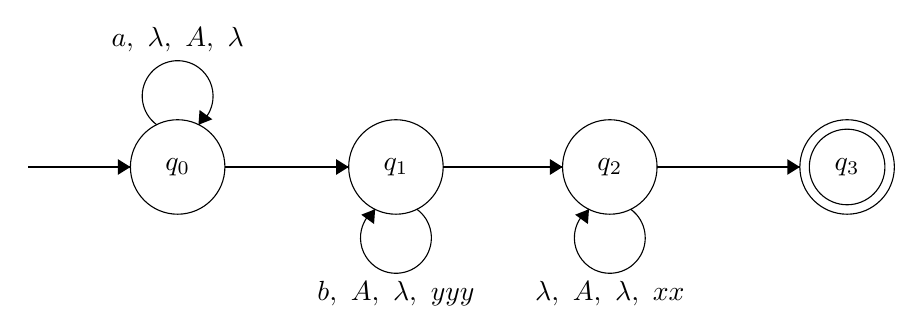
\begin{tikzpicture}[scale=0.2]
\tikzstyle{every node}+=[inner sep=0pt]
\draw [black] (15.349,-18.218) circle (3);
\draw (15.35,-18.22) node {$q_0$};
\draw [black] (29.209,-18.218) circle (3);
\draw (29.21,-18.22) node {$q_1$};
\draw [black] (42.791,-18.218) circle (3);
\draw (42.79,-18.22) node {$q_2$};
\draw [black] (57.86,-18.218) circle (3);
\draw (57.86,-18.22) node {$q_3$};
\draw [black] (57.86,-18.218) circle (2.4);
\draw [black] (14.026,-15.539) arc (234:-54:2.25);
\draw (15.35,-10.97) node [above] {$a,\mbox{ }\lambda,\mbox{ }A,\mbox{ }\lambda$};
\fill [black] (16.67,-15.54) -- (17.55,-15.19) -- (16.74,-14.6);
\draw [black] (32.21,-18.22) -- (39.79,-18.22);
\fill [black] (39.79,-18.22) -- (38.99,-17.72) -- (38.99,-18.72);
\draw [black] (45.79,-18.22) -- (54.86,-18.22);
\fill [black] (54.86,-18.22) -- (54.06,-17.72) -- (54.06,-18.72);
\draw [black] (18.35,-18.22) -- (26.21,-18.22);
\fill [black] (26.21,-18.22) -- (25.41,-17.72) -- (25.41,-18.72);
\draw [black] (30.532,-20.898) arc (54:-234:2.25);
\draw (29.21,-25.47) node [below] {$b,\mbox{ }A,\mbox{ }\lambda,\mbox{ }yyy$};
\fill [black] (27.89,-20.9) -- (27.01,-21.25) -- (27.82,-21.84);
\draw [black] (44.113,-20.898) arc (54:-234:2.25);
\draw (42.79,-25.47) node [below] {$\lambda,\mbox{ }A,\mbox{ }\lambda,\mbox{ }xx$};
\fill [black] (41.47,-20.9) -- (40.59,-21.25) -- (41.4,-21.84);
\draw [black] (5.86,-18.22) -- (12.35,-18.22);
\fill [black] (12.35,-18.22) -- (11.55,-17.72) -- (11.55,-18.72);
\end{tikzpicture}
\end{center}
